\documentclass{scrartcl}
\usepackage[utf8]{inputenc}
\usepackage{graphicx}%GRaphiken
\usepackage{tabularx}%Tabellen!
\usepackage[english]{babel}% Zeilentrennung besser
\usepackage{url}% Urls besser
\usepackage{textcomp}% Sonderzeichen
\usepackage{amsmath}%maths / equations
\usepackage{helvet}% Schrift Helvetica
% \usepackage[helvet]{sfmath}% Helvet also in Math modes
% \renewcommand\familydefault{\sfdefault}
\usepackage{sansmath} % sans in math
\usepackage[]{color}
\usepackage{booktabs} % for cmidrule
\usepackage{siunitx} % to aling column s on dots
\usepackage{todonotes}
\usepackage[
	left=3cm,
	right=2cm,
	top=1.5cm,
	bottom=1cm
	,
	includeheadfoot
	]{geometry}														% Satzspiegel
\usepackage[
	round,	%(defaultage in the main file and \input ) for round parentheses;
	%square,	% for square brackets;
	%curly,	% for curly braces;
	%angle,	% for angle brackets;
	colon,	% (default) to separate multiple citations with colons;
	%comma,	% to use commas as separaters;
	authoryear,% (default) for author-year citations;
	%numbers,	% for numerical citations;
	%super,	% for superscripted numerical citations, as in Nature;
	sort,		% orders multiple citations into the sequence in which they appear in the list of 				references;
	%sort&compress,    % as sort but in addition multiple numerical citations
                   % are compressed if possible (as 3-6, 15);
	%longnamesfirst,  % makes the first citation of any reference the equivalent of
                   % the starred variant (full author list) and subsequent citations
                   %normal (abbreviated list);
	%sectionbib,      % redefines \thebibliography to issue \section* instead of \chapter*;
                   % valid only for classes with a \chapter command;
                   % to be used with the chapterbib package;
	%nonamebreak,     % keeps all the authors names in a citation on one line;
                   %causes overfull hboxes but helps with some hyperref problems.
]{natbib}											    			% Literaturverzeichnis
\usepackage{scrhack}   % kills \float@addtolists!  warning
\usepackage[pdfpagelabels,plainpages=false, pageanchor=false]{hyperref}	


%% andere Einstellungen
\linespread{1.5}% 1.5 Zeilenabstand			
\graphicspath{{fig/}}                     % path to graphics


%% ----------------------------------------------------------------------------
\title{Ecotoxicology is not normal.}
\subtitle{How the use of proper statistical models can increase statistical power in ecotoxicological experiments.}
\author{Eduard Szöcs, Ralf B. Schäfer}
\date{\today}



%% ----------------------------------------------------------------------------
\begin{document}
\maketitle

\section*{Abstract}


%% --------------------------------
\section{Introduction}
In environmental risk assessments (ERA) statistical tests play an important role to evaluate the effects of pesticides. 
Despite criticism (e.g. \citet{landis_well_2011}) statistics like the No Observed Effect Concentration (NOEC) are still regularly used to report results experiments \citep{jager_bad_2012}. 
A critical issue of reporting a NOEC is the statistical power in the underlying experiments, i.e. the ability to detect an effect.

Ecotoxicologists perform various kinds of experiments yielding to different types of data, potentially with very low samples sizes. 
Examples are: animal counts in mesocosm experiments (positive, integer valued, discrete data), proportions of surviving animals (discrete, bonded between 0 and 1) or biomass in growth experiments (strictly positive data).

Such data are usually analysed by using methods assuming normal distributed data, although these types are inherently not normally distributed \citep{wang_making_2011}. 
In order to approximate the normality and variance homogeneity assumptions data is usually transformed.
It is advised that survival data can be transformed using an arcsine square root transformation \citep{oecd_current_2006, newman_quantitative_2012}. 
For count data from mesocosm experiments a log(Ax + 1) transformation is usually usually, where the constant A is either chosen arbitrarily or following the recommendation of \citet{van_den_brink_impact_2000}: Ax to be 2 for the lowest abundance value (x) greater than zero. 
Note, that there has been little evaluation and advice for the practitioners which transformations to use.
If the transformed data does not meet the normality assumptions, usually non-parametric tests are applied \citep{wang_making_2011}.

Generalized linear models (GLM) are a third possibility to analyse such not normally distributed data \citep{nelder_generalized_1972}.
GLMs can handle various types of data distributions, e.g. Poisson or negative binomial (for count data) or binomial (for discrete proportions); the normal distribution being a special case of GLMs.
Despite that GLMs were available more than 40 years now, ecotoxicologists do not regularly make use of them.

Recently studies concluded that data transformations should be avoided and GLMs be used as they have better statistical properties (\emph{Do not log-transform count data}, \citep{ohara_not_2010}; \emph{The arcsine is asinine}, \citep{warton_arcsine_2011}).
Especially in the light of low sample sizes, which are common in ecotoxicological studies \citep{sanderson_pesticide_2002,szocs_analysing_2015}, differences between statistical methods may be apparent. 

We first give two motivating examples showing that different methods may lead to different conclusions. 
% Then review what types of analysis are used by ecotoxicologists.
Then we compare three types of statistical methods (transformation and normality assumption, GLM, non-parametric tests) using simulations.


\section{Motivating examples}
\subsection{Count data}
\citet{brock_minimum_2014} provides a typical example data from a mesocosm study of mayfly larvae counts on artificial substrate samplers at one sampling day (Figure \ref{fig:example}). 
18 mesocosms have been sampled, with 6 treatments (Control, n = 4; 0.1 mg/L, 0.3mg/L, 1mg/l, 3mg/L, n = 3; 10 mg/L, n = 2).
We will use this data to demonstrate the differences between transformations, different GLMs and a non-parametric approach.

\subsubsection{The linear model}
To fit the standard linear model, we first transform the counts following \citet{van_den_brink_impact_2000}:

\begin{align}
  y^T_i & = log(Ay_i + 1) \label{eqn:trans} \\
  A & = 2~/~min(y)~~~~~\text{, for}~ y > 0 \nonumber
\end{align}

, where $y_i$ is the measured abundance, $y_i^T$ the transformed abundance and A = 2 / 11 = 0.182.

We fit the well known linear model:
\begin{align}
  y_i^T &\sim N(\mu_i, \sigma^2) \nonumber \\
  y_i^T &= \alpha + \beta x_i \label{eqn:normal} \\
  var(y_i^T) &= \sigma^2 \nonumber
\end{align}
This model assumes a normal distributed response with constant variance ($\sigma^2$).
Note, that we it parametrised as contrast ($\beta x_i$) to the control group ($\alpha$) so that the LOEC can be directly deduced from the estimates of $\beta$.


\subsubsection{Generalized Linear Models}
GLMs are the extension of the normal model, by allowing other distributions of the response variable.
Instead of transforming the response variable the counts could be directly modelled by a Poisson distribution:

\begin{align}
  y_i &\sim P(\lambda_i) \nonumber \\
  log(\lambda_i) &= \mu_i \label{eqn:pois} \\
  \mu_i &= \alpha + \beta x_i \nonumber \\
  var(y_i) &= \lambda_i \nonumber
\end{align}

Again, this model is parametrised as contrast to the control group. 
The expected values of y ($\lambda$) are linked with a log-function to the predictors, to avoid negative fitted values. 
The Poisson distribution assumes that the mean and the variance are equal - a assumption that is rarely met with ecological data which is typically characterized by greater variance (overdispersion).
To overcome this problem a quasi-Poisson distribution could be used which introduces an additional overdispersion parameter ($\Theta$):
\begin{align}
  y_i &\sim P(\lambda_i, \Theta) \label{eqn:quasi} \\
  % log~\lambda &= \mu \label{eqn:quasi} \\
  % \mu &= \alpha + \beta X \nonumber \\
  var(y_i) &= \Theta \lambda_i  \nonumber
\end{align}

Another possibility to deal with overdispersion is to use a negative binomial distribution:

\begin{align}
  y_i &\sim NB(\lambda, \kappa) \label{eqn:negbin}  \\
  % log~\lambda &= \mu \label{eqn:negbin} \\
  % \mu &= \alpha + \beta X \nonumber \\
  var(y_i) &= \lambda_i + \kappa \lambda_i^2 \nonumber
\end{align}

In both cases the parametrisation and link function is the same as in the Poission GLM.
Note, that the quasi-Poisson model assumes a linear mean-variance relationship, whereas the negative binomial model a quadratic relationship.
The above described models are most commonly used in ecology, although other distributions for count data are possible, like the negative binomial with a linear mean variance relationship (also known as NB1) or the poisson inverse gaussian \citep{hilbe_modeling_2014}.


\subsubsection{Hypothesis testing}

On this data, we could test different hypotheses like (i) if is there any effect of the treatment or (ii) test single parameters (treatments) to determine the LOEC.
We used F-tests for the normal and quasi-Poisson models and Likelihood-Ratio (LR) tests for Poisson and negative binomial models to test if there is any treatment related effect.
To assess the LOEC we used Dunnett contrasts with one-sided Wald t tests (normal and quasi-poisson) and one-sided Wald Z tests (Poisson and negative binomial) following general recommendations \citep{bolker_generalized_2009}. 
% Moreover, we used parametric bootstrap (with 2000 bootstrap samples) to assess the LR and parameters in the negative binomial model \citep{faraway_extending_2006}.
% For comparison, we also performed the commonly used non-parametric Kruskal-Wallis test and pairwise Wilcoxon test on untransformed data.
% P-values from multiple comparisons where adjusted using the method of \citet{holm_simple_1979}.


\subsubsection{Results}
The Poisson model showed considerable overdispersion and did not fit to the data. Therefore, inferences are not valid and we do not further discuss it's results. \todo{see supplement}
The normal (F = 2.57, p = 0.084) and quasi-Poisson model (F = 2.90, p = 0.061) did not indicate any treatment related effects.
Whereas the LR test of the negative binomial model indicated a treatment related effect (LR = 13.99, p = 0.016).

All methods resulted in similar predicted values, except the normal model predicting always lower abundances (Figure \ref{fig:example}). 
95\% Confidence intervals (CI) where most narrow for the negative binomial model and widest for quasi-Poisson - especially at lower estimated abundances.
Accordingly, the determined LOECs differed (Normal and quasi-Poisson: 3 mg/L, negative binomial: 0.3 mg/L).

\citet{brock_minimum_2014} assumed normality after data transformation and reported a LOEC of \mbox{0.3 mg/L} for this data.
The reason for this difference may be twofold: \citep{brock_minimum_2014} used a $log(2~y + 1)$ transformation, whereas we used a $log(0.182~y + 1)$ transformation \citep{van_den_brink_impact_2000}.
Moreover, we applied a one-sided Dunnett test, as the toxic response in a mesocosm experiment may be either decreasing or increasing (due to biological interactions).
\citet{brock_minimum_2014} used a one-sided Williams test, which is known to have larger power if the assumptions are met \citep{jaki_statistical_2013}.
This example demonstrates that the choice of the statistical model and procedure might have tremendous impact on ecotoxicological inferences, especially when sample sizes are low.

\begin{figure}[h]
  \centering
  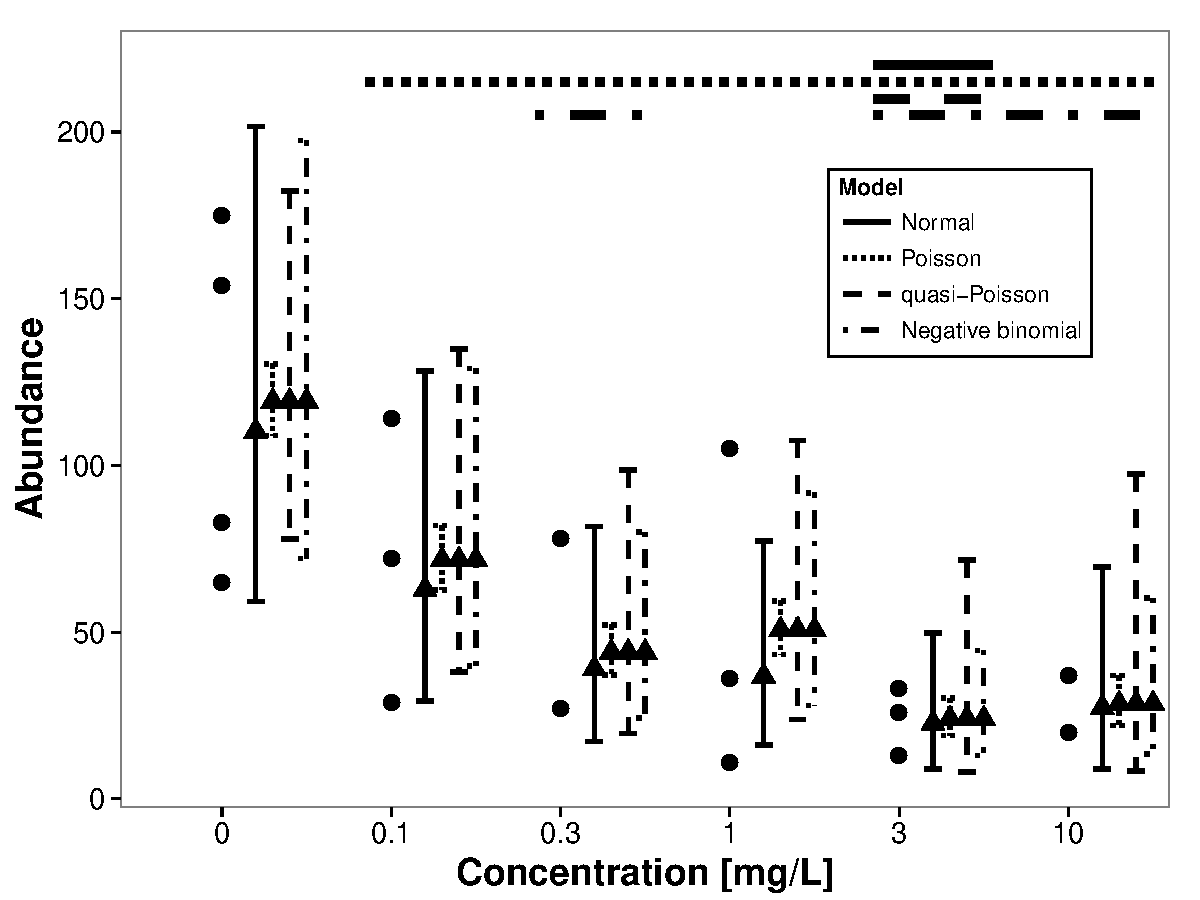
\includegraphics[width = 0.8\textwidth]{example.pdf}
  \caption{Data from \citet{brock_minimum_2014} (boxes + black points) and estimates + 95\% Wald Z or t Confidence intervals from the fitted models (vertical lines). 
  Bars above indicate treatments statistically significant different from the control group (Dunnett contrasts).}
  \label{fig:example}
\end{figure}


\subsection{Binomial data}
\citet{weber_short-term_1989} provides fathead minnow \textit{Pimephales promelas} larval survival data after sodium pentachlorophenol (NaPCP) exposure.
This data was also exemplary analysed in \citet{newman_quantitative_2012}.
At six NaPCP concentrations (0, 32, 64, 128, 256, 512 \textmu g/L) with 4 replications ten fish were exposed and proportions of total number alive at the end reported.

\subsubsection{The linear model after transformation}
To accommodate the assumption for the standard linear model the EPA suggests a arcsine square root transformation for such kind of data \cite{epa_methods_2002}:

\begin{align}
  y_i^T = 
  \begin{cases}  
    arcsin(1) - arcsin(\sqrt{\frac{1}{4N}}) & \text{, if}\ y_i = 1 \\
    arcsin(\sqrt{\frac{1}{4N}}) & \text{, if}\ y_i = 0  \\
    arcsin(\sqrt{y_i}) & \text{, otherwise}
  \end{cases} \label{eqn:arcsine}
\end{align}

, where $y_i^T$ are the transformed proportions and N is the number of exposed animals.
The transformed proportions are then analysed using the standard linear model (see above).

\subsubsection{Generalized Linear Models}

Data of type \emph{x out of n} are typically modelled by a binomial distribution with parameters N and $\pi$:

\begin{align}
  y_i &\sim Bin(N, \pi_i) \nonumber \\
  logit~(\pi_i) &= \alpha + \beta x_i \label{eqn:bin} \\
  var(y_i) &=  \pi_i (1 - \pi_i) / N \nonumber
\end{align}

, with N = number of exposed animals and $\pi$ is the probability of survival.
The variance of the binomial distribution is a quadratic function of the mean.

We used F-test for the normal and LR test for binomial GLM to determine a general treatment effect.
LOEC was assessed using one-sided Dunnett contrasts.


\subsubsection{Results}
For this dataset, both methods yielded to same ecotoxicological inferences:
The global tests of both methods indicated a strong effect of NaPCP on larval survival (linear model: F = 13.31, p \textless 0.001; GLM: LR = 64.79, p \textless 0.001).
Moreover, both methods identified the highest concentration (512 \textmu g/L) as LOEC. 
However, the coefficients of the binomial model are directly interpretable as change in the odds ratio, whereas this is not possible with the transformed data (Table \ref{tab:ex_bin}).

\begin{table}[h]
\centering
\footnotesize
\caption{Estimated parameters and 95\% Confidence Intervals for the binomial data example. 
Asterisks indicate LOEC as determined using one-sided Dunnett tests.}
\label{tab:ex_bin}
\begin{tabular}{lS[table-format=3.2]lS[table-format=3.2]l}
\hline
 & \multicolumn{4}{c}{Model} \\ 
Parameter & \multicolumn{2}{c}{LM} & \multicolumn{2}{c}{GLM} \\ 
\cmidrule(lr){2-3} \cmidrule(lr){4-5} 
Control ($\alpha$) & 1.331 & (1.180, 1.481) & 2.994 & (1.523, 4.366) \\ 
32 \textmu g/L  & -0.147 & (-0.360, 0.066) & -1.21 & (2.876, 0.456) \\ 
64 \textmu g/L  & 0.041 & (0.172, 0.254) & 0.719 & (-1.723, 3.161) \\ 
128 \textmu g/L  & -0.076 & (0.289, 0.137) & -0.747 & (-2.505, 1.010) \\ 
256 \textmu g/L & -0.221 & (-0.434, -0.008) & -1.708 & (-3.312, -0.104) \\ 
512 \textmu g/L  & -0.727 & (-0.941, -0.514)$*$ & -3.675 & (-5.244, -2.107)$*$ \\ 
\hline
\end{tabular}
\end{table}



\section{Simulations}
We used simulations to compare the methods described above to analyse count and binomial data.
Methods were compare in terms of Type I error (maintain a significance level of 0.05 when there is no effect) and power (detect an effect when it is present). 
We fitted the models and tested hypotheses on the simulated data as described in the motivating example.

All simulations were done in R (Version 3.1.2) on a 64-bit Linux machine with 8 GB and 2.2 GHz.
Exemplary analysis of data in the motivating example can be found in the supplement.
Source code for the simulations is available online at \url{https://github.com/EDiLD/usetheglm}. \todo{git repo currently private -> tidy}

\subsection{Count data}
\subsubsection{Methods}
We simulated count data that mimics count data encountered in mesocosm experiments, with five treatments (T1 - T5) and one control group (C).
Counts were drawn from a negative binomial distribution with slight over dispersion (dispersion parameter for all treatments: $\kappa = 0.25$).
We simulated datasets with different number of replicates (N = \{3, 6, 9\}) and different abundances in control treatments ($\mu_\text{\tiny C}$ = \{2, 4, 8, 16, 32, 64, 128\}). 
For power estimation mean abundance in treatments T2 - T5 was reduced to half of control and T1 ($\mu_\text{\tiny T2}~=~...~=~\mu_\text{\tiny T5}~=~0.5~\mu_\text{\tiny C} = 0.5~\mu_\text{\tiny T1}$), resulting to a theoretical LOEC at T2.
For Type I error estimation mean abundance was kept equal between all groups.

For each combination we generated 100 datasets. 
We fitted a linear model after log (Ax + 1) transformation ($LM$), negative binomial GLM ($GLM_{nb}$) and quasi-Poisson GLM ($GLM_{qp}$) to this datasets. 

We tested a general treatment effect using F tests ($LM$ and $GLM_qp$) and LR tests ($GLM_nb$). Additionally, we applied used parametric boostrap to assess the LR in the negative binomial model ($GLM_pb$) and used a Kruskal-Wallis test on untransformed data as non-parametric method.

Moreover, we compared the methods ability to determine the LOEC (T2 in our simulation design).

\todo{hier noch besser machen!}
As our simulation
We used one-sided Dunnett tests 
 by comparing inferences on model parameters and using pairwise Wilcoxon test as non-parametric method.

\subsubsection{Results}
For this simulation design (reduction in abundance by 50\%) a sample size of n = 9 was needed to achieve a power greater then 80\%.
For small sample sizes (n = {3, 6}) and low abundances ($\mu_C$ = {2, 4}) many of the negative binomial models ($GLM_{nb}$ and $GLM_{pb}$) did not converge to a solution (convergence rate \textless 80\% of the simulations). \todo{Supplement Convergence table.}

$GLM_{nb}$ showed an increased Type I error at low sample sizes for the test of treatment effect. 
However, this decreased to an acceptable limit with increasing sample sizes (Figure \ref{fig:p_glob_c}, bottom).
$LM$, $GLM_{qp}$ and $GLM_{pb}$ maintained an appropriate Type I error, with $GLM_{qp}$ having greatest power.
The Kruskal-Wallis test showed least power, with low Type I error at small sample sizes. 
At bigger sample sizes (n = 9) all GLM had higher power than LM or the Kruskal test (Figure \ref{fig:p_glob_c}). 

\begin{figure}[h]
  \centering
  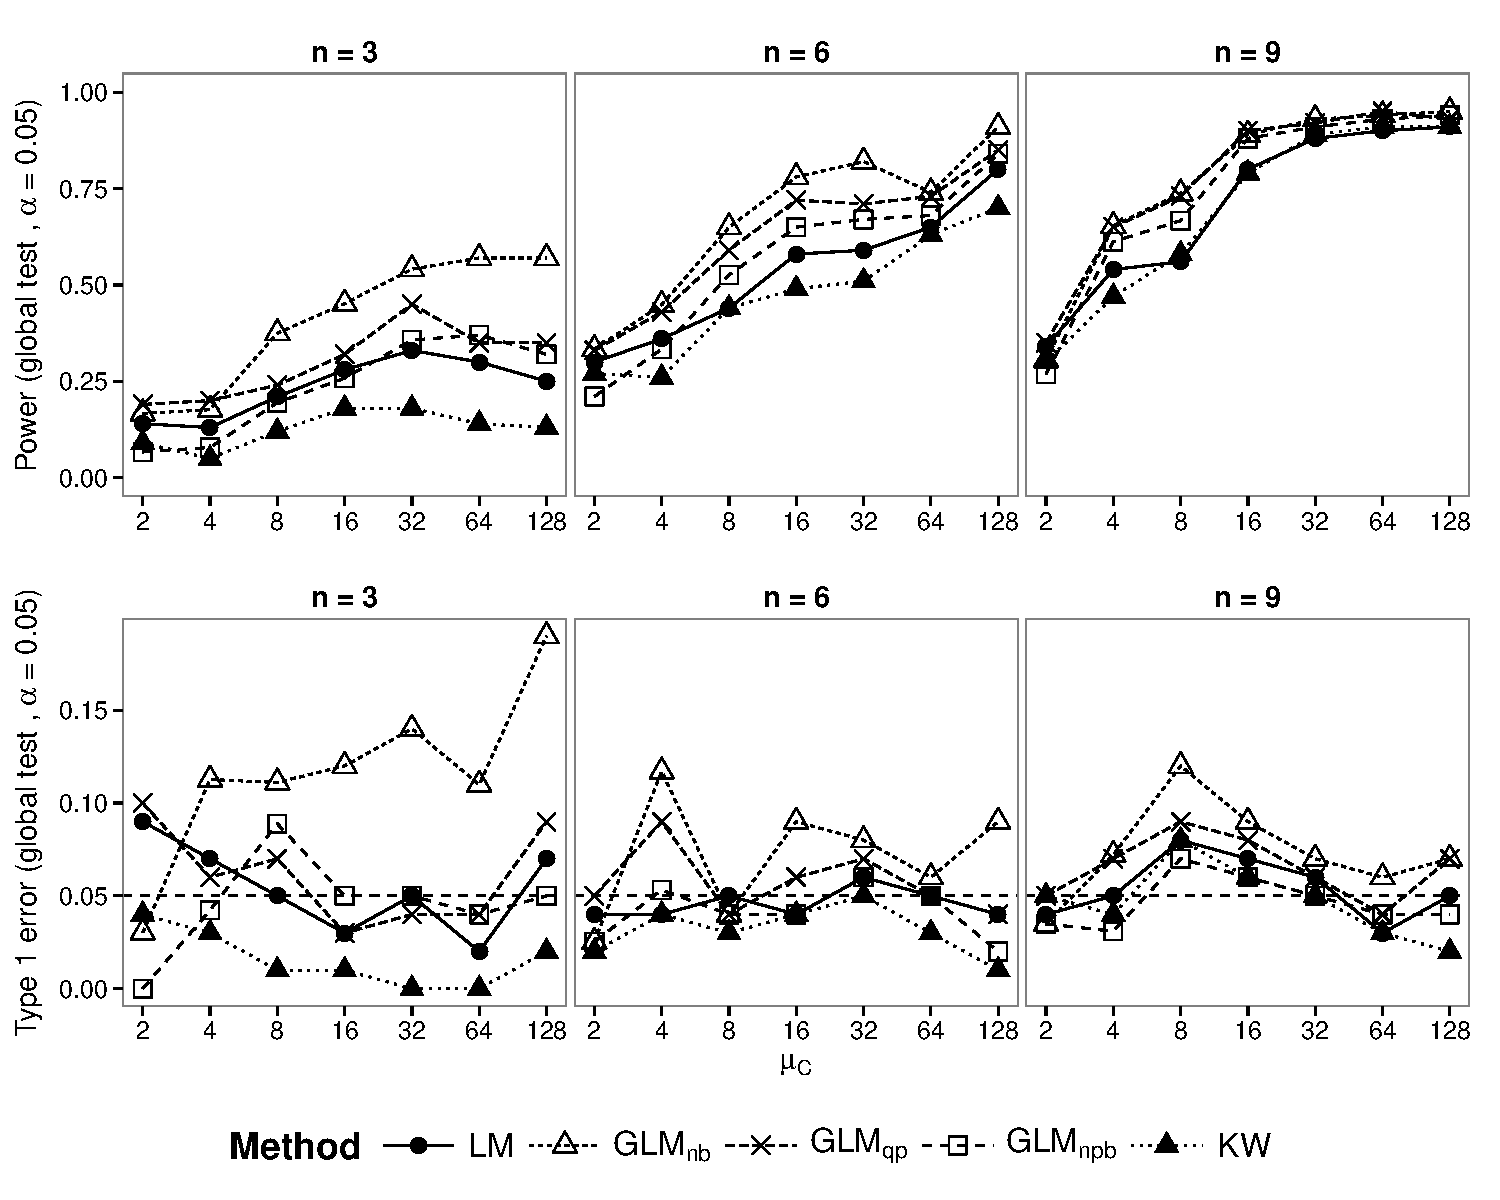
\includegraphics[width = 0.8\textwidth]{p_glob_c.pdf}
  \caption{Simulation results for count data. Power (top) and Type I error (bottom) for the test of a treatment effect. Compared methods were: Linear model after log (Ax + 1) transformation (lm), negative binomial GLM with LRT (glm\_nb), negative binomial GLM with parametric boostrap (glm\_pb), quasi-Poisson GLM (glm\_qp) and Kruskal-Wallis test on untransformed data (np).
  For n = 3 and $\mu_C$ = {2, 4} less then 80\% of glm\_nb and glm\_pb models did converge.}
  \label{fig:p_glob_c}
\end{figure}

The inferences on parameters showed up to 87\% less power compared to the test of a general treatment effect (excluding $\mu_C$ = \{2, 4\} due to convergence problems and the pairwise wilcox test; Figures \ref{fig:p_glob_c} and \ref{fig:p_loec_c}).
The pairwise Wilcoxon Test had no power at all to detect the correct LOEC.
$GLM_{nb}$ and $GLM_{pb}$ showed an increased Type 1 error at low sample sizes and $GLM_{qp}$ beeing slightly conservative.
$GLM_{pb}$ and $LM$ yielded to comparable power.

\begin{figure}[h]
  \centering
  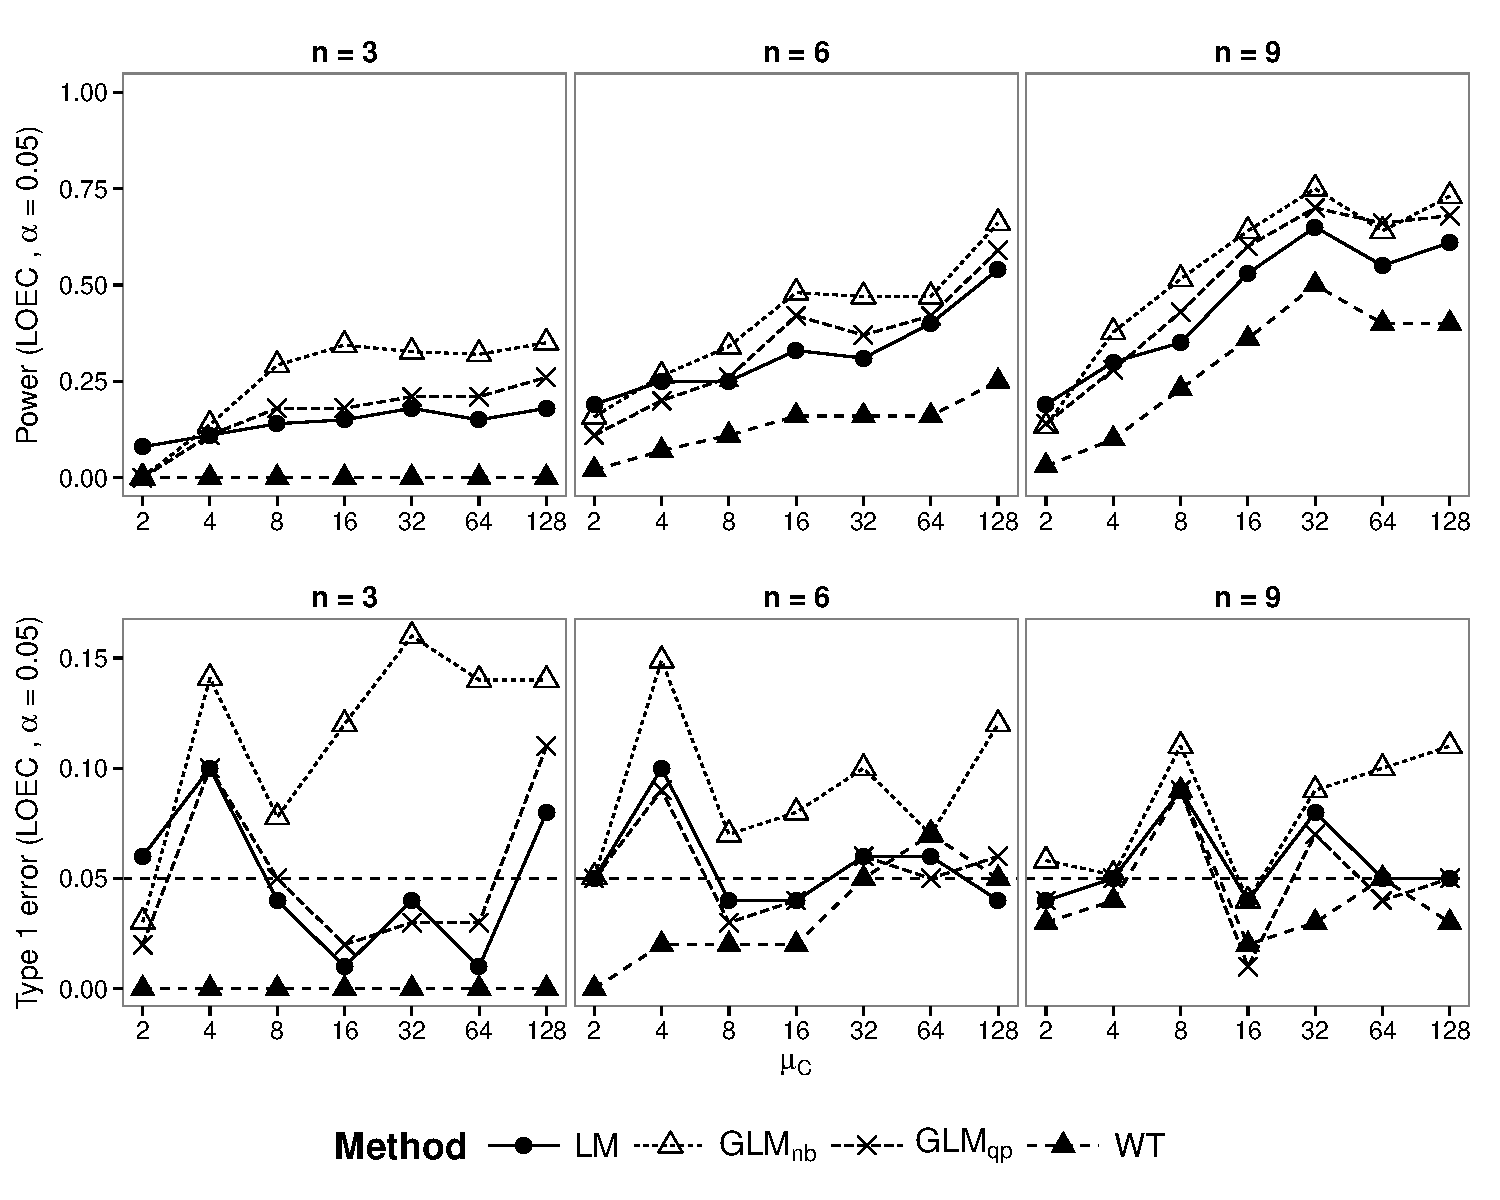
\includegraphics[width = 0.8\textwidth]{p_loec_c.pdf}
  \caption{Simulation results for count data. Power (top) and Type I error (bottom) for determination of LOEC. Compared methods were: Linear model after log (Ax + 1) transformation (lm), negative binomial GLM with LRT (glm\_nb), negative binomial GLM with parametric boostrap (glm\_pb), quasi-Poisson GLM (glm\_qp) and pairwise Wilcoxon test on untransformed data (np). For n = 3 and $\mu_C$ = {2, 4} less then 80\% of glm\_nb and glm\_pb models did converge.}
  \label{fig:p_loec_c}
\end{figure}



\subsection{Binomial data}
\subsubsection{Methods}
We simulated data from a design as described in the motivating example, with 5 treated (T1 - T5) and a control group (C). 
Proportions were drawn from a Bin(10, $\pi$) distribution, with varying probability of success ($\pi$ = \{0.60, 0.65, 0.70, 0.75, 0.80, 0.85, 0.90, 0.95\}) and varying number of replicates (N = \{3, 6, 9\}).
For Type I error estimation $\pi$ was held constant between groups.
For power estimation $\pi$ in C and T1 was set to 0.95 and $\pi$ in T2 - T5 varied between 0.6 and 0.95). 
 
We simulated 250 datasets for each combination and analysed them using the linear model after arcsine transformation (LM), binomial GLM (GLM) and Kruskal-Wallis test.
Moreover, we compared the methods ability to determine the LOEC (T2 in our simulation design) by comparing inferences on model parameters and a pairwise Wilcoxon test. 


\subsubsection{Results}
At low samples sizes the binomial GLM showed greatest power for testing the treatment effect, while maintaining an appropriate Type I error level.
Kruskal-Wallis test had lowest power and a low Type I error rate.
However, the difference between methods quickly vanished with increasing samples sizes (Figure \ref{fig:p_glob_p}).

\begin{figure}[h]
  \centering
  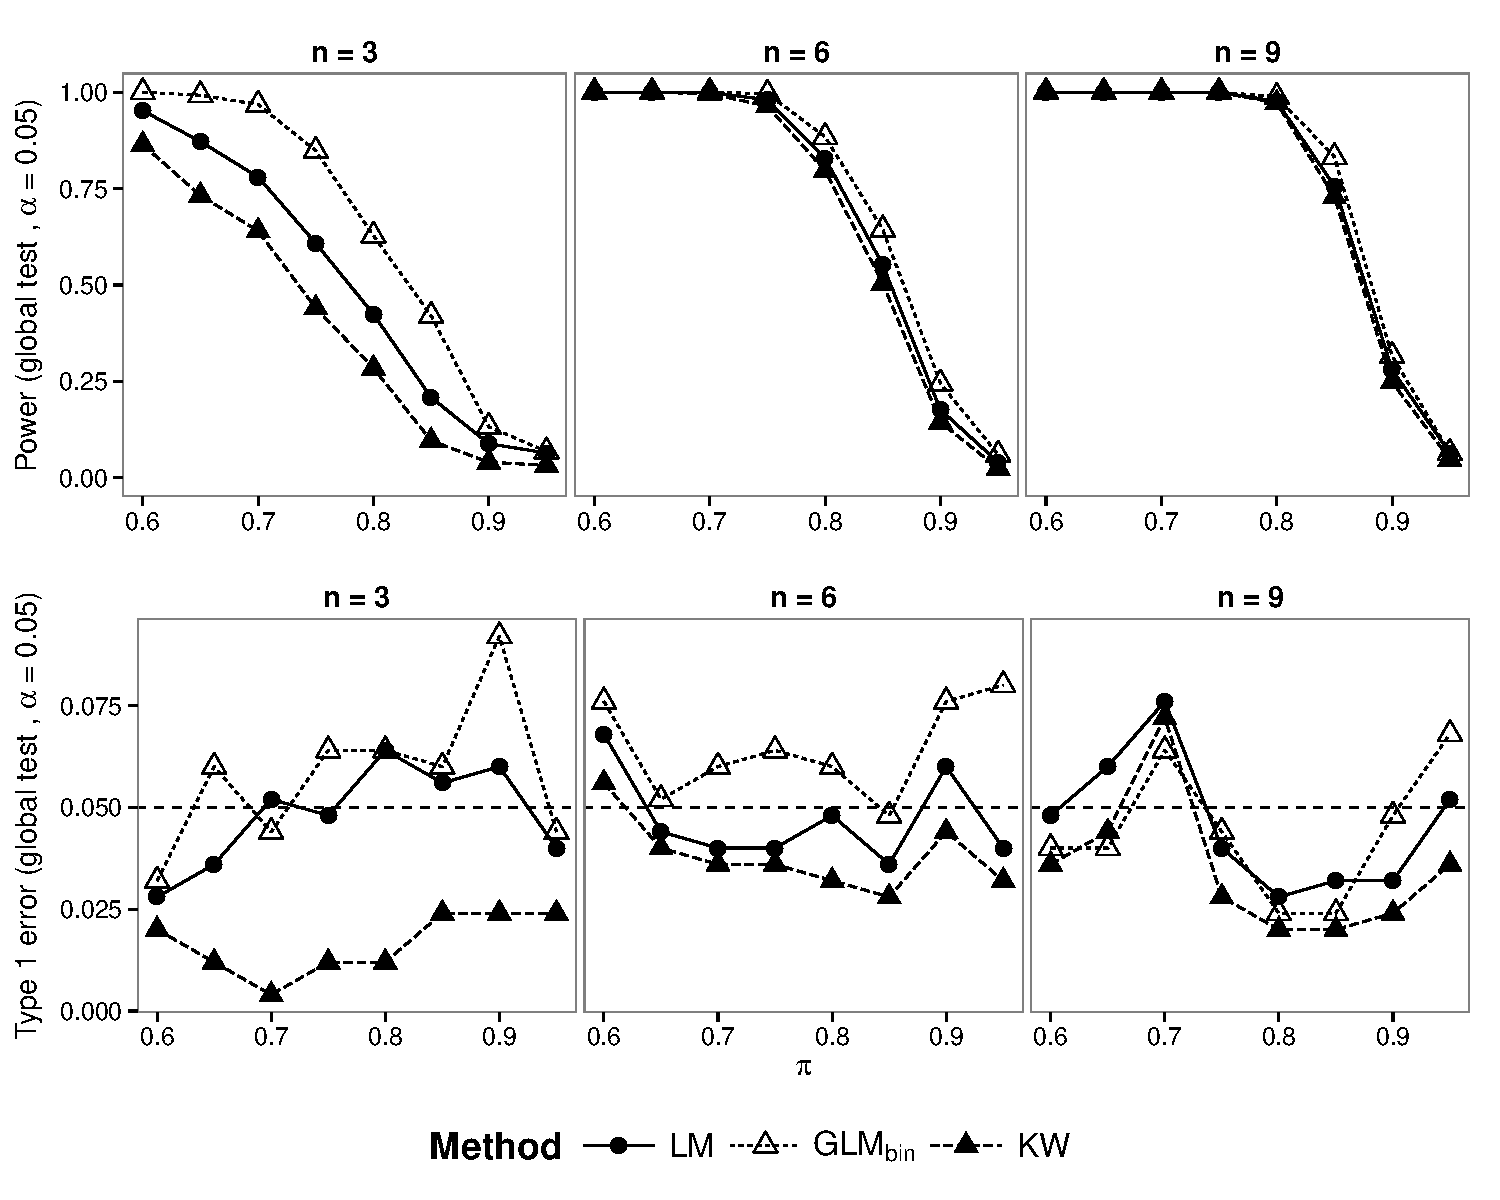
\includegraphics[width = 0.8\textwidth]{p_glob_p.pdf}
  \caption{Simulation results for binomial data. Power (top) and Type I error (bottom) for the test of a treatment effect. Compared methods were: Linear model after arcsine square root transformation (lm), binomial GLM with LRT (glm) and Kruskal-Wallis test on untransformed data.}
  \label{fig:p_glob_p}
\end{figure}

Inference on parameters was not as powerful as inference on the general treatment effect.
For small sample sizes LM showed highest power, while maintaing a Type 1 error level of 0.05.
GLM had less power and showed a low Type 1 error rate, especially with decreasing effect size.
The pairwise Wilcoxon test had no power at all for n = 3.
The differences in power to detect a LOEC vanished quickly with increasing sample sizes (Figure \ref{fig:p_loec_p}). 

\begin{figure}[h]
  \centering
  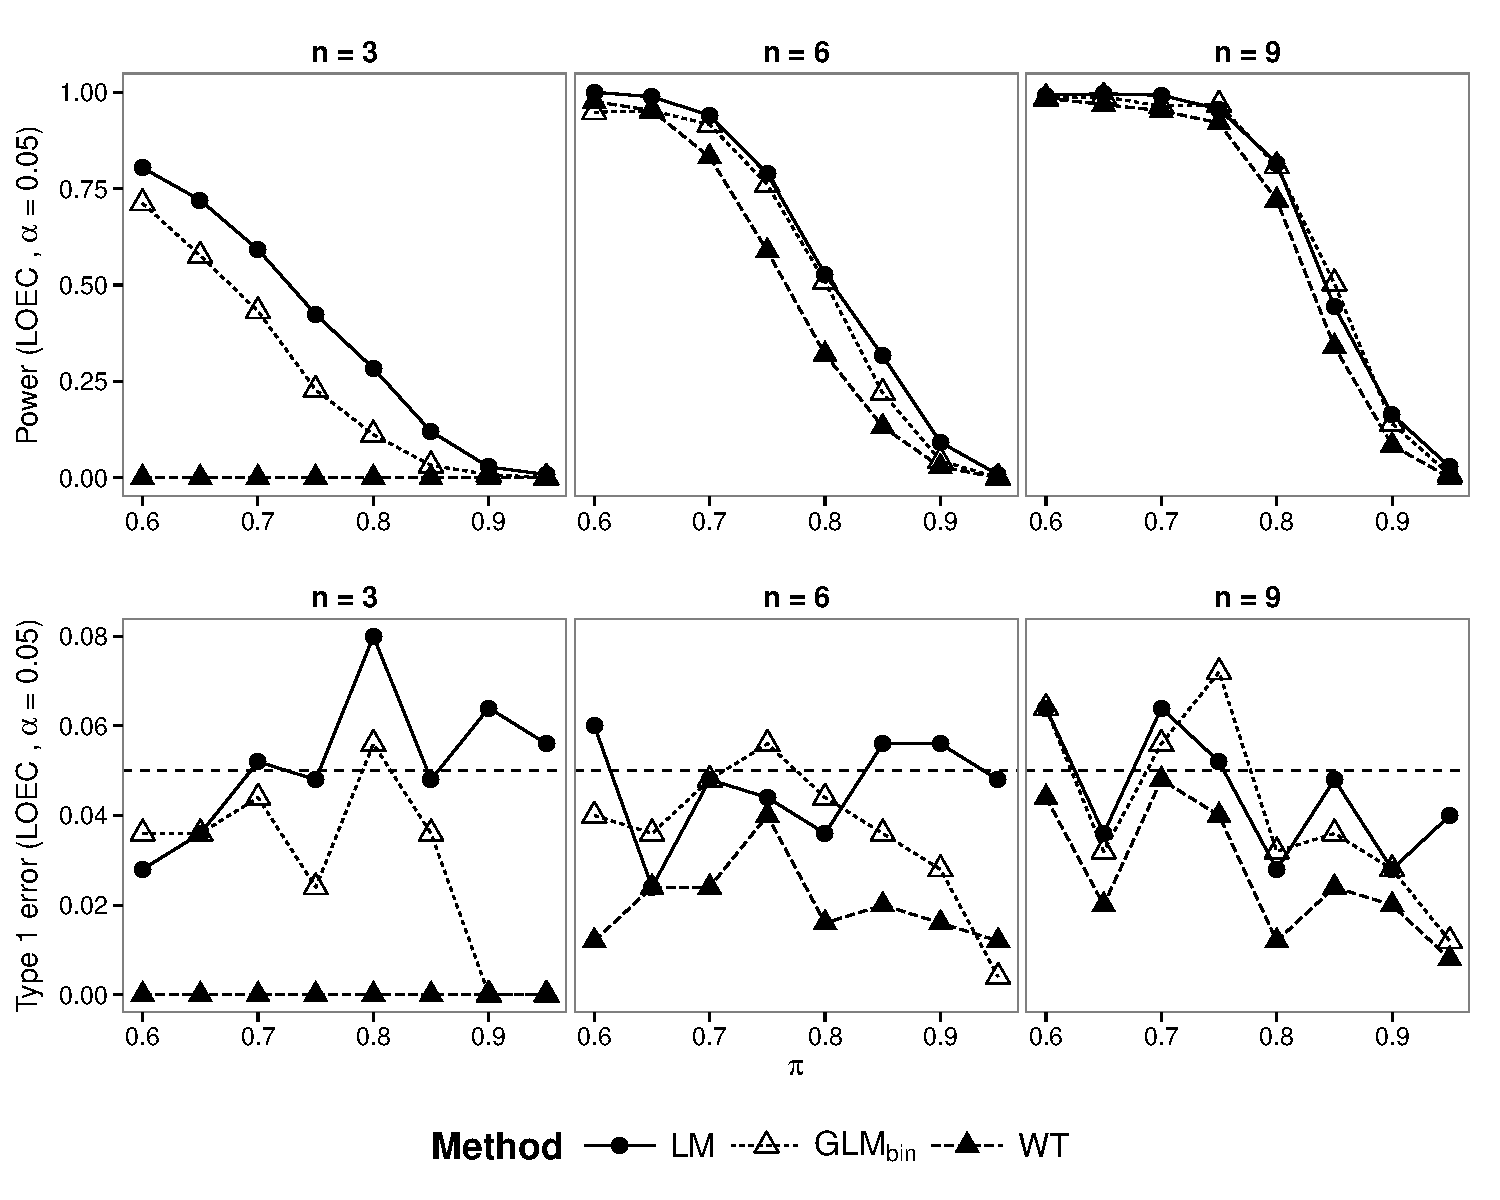
\includegraphics[width = 0.8\textwidth]{p_loec_p.pdf}
  \caption{Simulation results for binomial data. Power (top) and Type I error (bottom) for determination of LOEC. Compared methods were: Linear model after arcsine square root transformation (lm), binomial GLM with LRT (glm) and Kruskal-Wallis test on untransformed data.}
  \label{fig:p_loec_p}
\end{figure}



\section{Discussion}
Statistical hypothesis tests are commonly used to make ecotoxicological inferences. 
Often these inferences are based on experiments with small sample sizes due to practical contraints.
\todo{Überleitung}

We showed for two common data types in ecotoxicology, that using an appropriate model yielded higher statistical power, than trying to meet the assumptions of normality and variance homogeneity using transformations. 
How should one choose 

%% --- Normality testing - choosing the correct model

%% -- GLM / LR test not so good for low sample sizes.

%% --- Multivariate + GLMM -------
Although, our simulations covered only simple experimental designs, these findings may also extend to more complex designs. 
Nested or repeated designs with non-normal data could be analysed using Generalized Linear Mixed Models (GLMM) and may have advantages with respect to power \citep{stroup_rethinking_2014}.
For community analyses \emph{GLM for multivariate data} have been proposed as alternative to Principal Response Curves (PRC) and yielded to similar inferences, but better indication of responsive taxa \citep{warton_distance-based_2012,szocs_analysing_2015}.

%% --- Non-parametric
It has been advocated that, in the typical case of small sample sizes (n \textless 20) and non-normal data, non-parametric tests perform better than parametric tests assuming normality \citep{wang_making_2011}.
In contrast our results showed that the often applied Kruskal test and pairwise Wilcoxon test have equal or less power compared to tests assuming normality after data transformation.
GLM always performed better than non-parametric tests. 
However, there might be more powerful non-parametric tests available \citep{konietschke_rank-based_2012}.
Non-parametric statistics are focussing on testing, but not on estimation of effects.
GLM allows the estimation, additional to testing, and the interpretation of effects that might not be statistically significant, but ecologically relevant.
Therefore, we do not advise to use non-parametric tests for non-normal data, but instead use GLMs.

%% --- general low power
Extremely low samples sizes (n \textless 5) are common in mesocosm experiments \citep{sanderson_pesticide_2002,szocs_analysing_2015}.
We simulated a reduction of 50\% in abundance and with such low sample sizes power to detect a treatment effect was unacceptably low (\textless 50\% for methods with appropriate Type 1 error, Figure \ref{fig:p_glob_c}).
This is even worse for detecting the correct LOEC with power less than 15\%.
Although, the use of LOEC/NOEC has been heavily criticized in the past \citep{landis_well_2011}  they are still regularly used in ecotoxicology \citep{jager_bad_2012}, especially in mesocosm studies NOEC calculations are used in the majority of mesocosm experiments \citep{brock_minimum_2014,efsa_ppr_guidance_2013}.
% lesen honing, brock EFSA etc. aufpassen!
% Auf MDD eingehen!
% 50% reduction = class 4 for MDD (small effects can be determined?! - check)
Our results suggest, that



%% Convergence MASS glm.nb not best algorithm





\todo{How to choose models? MV plot,...}
\todo{robust SE for lower T1 error in glm nb?}
\todo{Kritik an NOEC}

\section{Conclusions}


\bibliography{references}
\bibliographystyle{apalike}

\end{document}
